\section{Constraint Satisfaction Programming - CSP}
In the context of Artificial Intelligence, a \textit{constraint satisfaction} is the process of finding a solution to a set of constraints that impose conditions that the variables must satisfy. A solution to a such a program is a set of values to be assigned to the variables that satisfies all the constraints defined. As \textit{modeling language} we have chosen \textbf{MiniZinc} to express variables and constraints of the mentioned problem.

\subsection{Minizinc Implementation}
The MiniZinc implementation follows closely the logical formulation presented in \S\ref{models}.

\paragraph{Input formatting}
Each instance of VLSI is presented as a .dzn file. The first line denotes the width of the silicon plate \texttt{width}, the second line the number of circuits to place \texttt{n\_circuits} and lastly there is a bi-dimensional array \texttt{dims} that defines the dimensions of each circuit.

\subsection{Without rotation}
To implement the model described in \S\ref{subsubsec:base-without-rot} we propose the following variable organization:
\begin{itemize}
    \item \textbf{Parameters}, which is the data given in input, then expressed in the MiniZinc language. In this section, we have defined the \texttt{max\_height} and \texttt{min\_height} which are the result of the aforementioned functions.
    \item \textbf{Decision Variables}, we have two decision variables, namely the variables that we would like to assign a value:
        \begin{itemize}
            \item the coordinates of each rectangle are gathered in an array \texttt{corner\_coords} where for a generic row \textit{c}, \texttt{corner\_coords[c, 1]} denotes the horizontal coordinate and \texttt{corner\_coords[c, 2]} denotes the vertical coordinate.
            \item the height of the silicon plate, \texttt{height}.
        \end{itemize}
\end{itemize}

\subsubsection{Simplest model}\label{simplest_model}
The only auxiliary function here is the one that computes the height and the corresponding constraints are listed here.
\begin{center}
    \begin{lstlisting}[language=Mzn]\label{simplest_mzn}
% No-overlap constraint
constraint forall(i,j in CIRCUITS where i!=j)(
  corner_coords[i,1] + dims[i,1] <= corner_coords[j,1] \/
  corner_coords[i,1] - dims[j,1] >= corner_coords[j,1] \/
  corner_coords[i,2] + dims[i,2] <= corner_coords[j,2] \/
  corner_coords[i,2] - dims[j,2] >= corner_coords[j,2]
);

% x, y of each block should have as starting coordinate (0,0)
constraint forall(i in CIRCUITS)(corner_coords[i, 1] >= 0);
constraint forall(i in CIRCUITS)(corner_coords[i, 2] >= 0);

% Boundaries constraint
constraint forall(i in CIRCUITS)(corner_coords[i, 1] + dims[i, 1] <= width);
constraint forall(i in CIRCUITS)(corner_coords[i, 2] + dims[i, 2] <= height);

% Height domain constraint
constraint height >= min_height /\ height <= max_height;

    \end{lstlisting}
\end{center}
\subsubsection{With global constraints}\label{global1}
In order to improve the performance of the previous model we have to introduce some \textit{global constraints} in the code. The most obvious above all is \texttt{diffn} which constrains each rectangle to be non-overlapping given its origin and sizes. First of all we have to remove the \textit{no-overlap} constraint from the previous model and add the following:
\begin{lstlisting}[language=Mzn]
constraint diffn([corner_coords[i, 1] | i in CIRCUITS], [corner_coords[i, 2] | i in CIRCUITS], [dims[i, 1] | i in CIRCUITS], [dims[i, 2] | i in CIRCUITS]);  
\end{lstlisting}
Another substantial improvement could be obtained by adding the \texttt{cumulative} for each one of the axes, specifically we are requiring that a set of tasks given by start times \textbf{s}(namely the array of $x_i$'s), durations \textbf{d}(namely the array of the horizontal sizes), and resource requirements \textbf{r}(namely the array of the vertical sizes), never require more than a global resource bound \textbf{b}(namely \textit{height}) at any one time. A similar reasoning can be done for the other axes. Said that we can simply add below the \texttt{diffn} constraint the following:
\begin{lstlisting}[language=Mzn]
constraint cumulative([corner_coords[i, 1] | i in CIRCUITS], [dims[i, 1] | i in CIRCUITS], [dims[i, 2] | i in CIRCUITS], height);            
constraint cumulative([corner_coords[i, 2] | i in CIRCUITS], [dims[i, 2] | i in CIRCUITS], [dims[i, 1] | i in CIRCUITS], width);  
\end{lstlisting}

\subsection{With rotation}
As we saw in \S\ref{subsubsec:base-rot}, we have to introduce in the MiniZinc model a new uni-dimensional array \texttt{rot} that tells us if a generic circuit is rotated by 90° or not. Therefore the constraints of the model proposed in \S\ref{simplest_model} can be easily modified in such a way:
\begin{lstlisting}[language=Mzn]
% No-overlap constraint
constraint forall(i,j in CIRCUITS where i != j)(
  corner_coords[i,1] + rot[i] * dims[i,2] + (1 - rot[i]) * dims[i,1] <= corner_coords[j,1] \/
  corner_coords[i,1] - rot[j] * dims[j,2] - (1 - rot[j]) * dims[j,1] >= corner_coords[j,1] \/
  corner_coords[i,2] + rot[i] * dims[i,1] + (1 - rot[i]) * dims[i,2] <= corner_coords[j,2] \/
  corner_coords[i,2] - rot[j] * dims[j,1] - (1 - rot[j]) * dims[j,2] >= corner_coords[j,2]
);

% Boundaries constraint
constraint forall(i in CIRCUITS)(corner_coords[i, 1] + rot[i] * dims[i,2] + (1 - rot[i]) * dims[i,1] <= width);
constraint forall(i in CIRCUITS)(corner_coords[i, 2] + rot[i] * dims[i,2] + (1 - rot[i]) * dims[i,1] <= height);

% Height domain
constraint height >= min_height /\ height <= max_height;

% Rot domain
constraint forall(i in CIRCUITS)(rot[i] >= 0 /\ rot[i] <= 1);
\end{lstlisting}

\subsubsection{With global constraints}
What we have done in \S\ref{global1} is basically the same here, the only thing is that we have to properly consider the possibility of rotation and so the fact that in \texttt{diffn} the sizes can change.
\begin{lstlisting}[language=Mzn]
constraint diffn([corner_coords[i, 1] | i in CIRCUITS], [corner_coords[i, 2] | i in CIRCUITS], [(1 - rot[i]) * dims[i, 1] | i in CIRCUITS], [rot[i] * dims[i, 2] | i in CIRCUITS]);

constraint cumulative([corner_coords[i, 1] | i in CIRCUITS], [dims[i, 1] | i in CIRCUITS], [dims[i, 2] | i in CIRCUITS], height);            
constraint cumulative([corner_coords[i, 2] | i in CIRCUITS], [dims[i, 2] | i in CIRCUITS], [dims[i, 1] | i in CIRCUITS], width);   
\end{lstlisting}

\subsection{Symmetry breaking}
Symmetry is an issue with the problem we are considering: for each solution there exists other seven symmetric variants: rotation by 90°, 180° and 270° and their respective vertically flipped versions (see figure \ref{fig:symmetries}).
\begin{figure}[!h]
\begin{center}$
\begin{array}{cc}
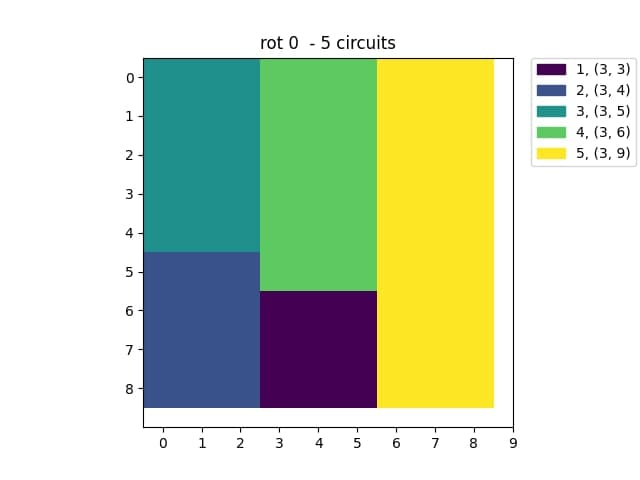
\includegraphics[width=2.5in]{images/sym_example/original.jpg} &
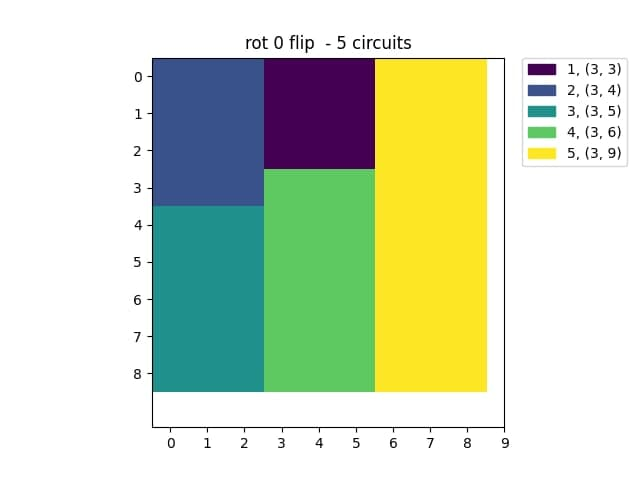
\includegraphics[width=2.5in]{images/sym_example/original_flipped.jpg} \\
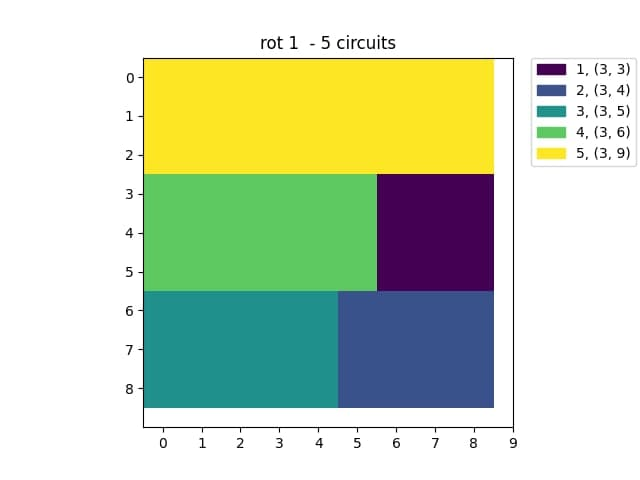
\includegraphics[width=2.5in]{images/sym_example/90.jpg} &
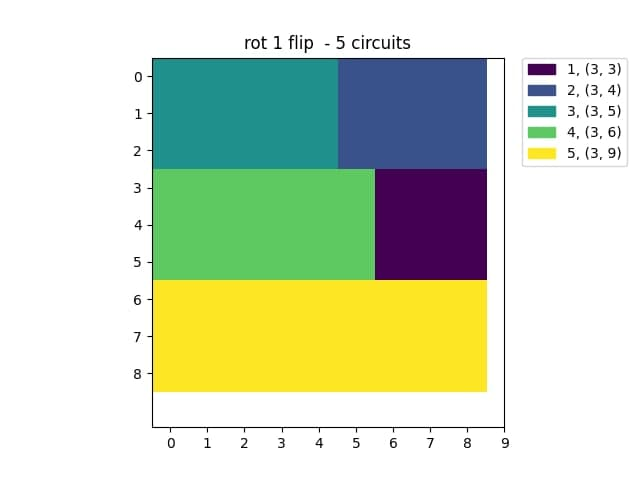
\includegraphics[width=2.5in]{images/sym_example/90_flipped.jpg} \\
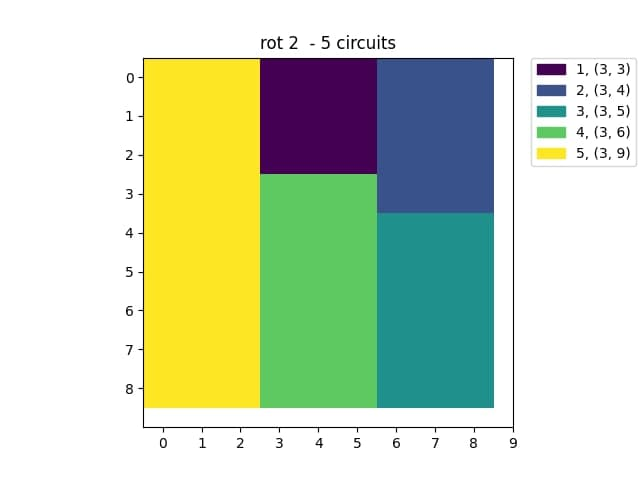
\includegraphics[width=2.5in]{images/sym_example/180.jpg} &
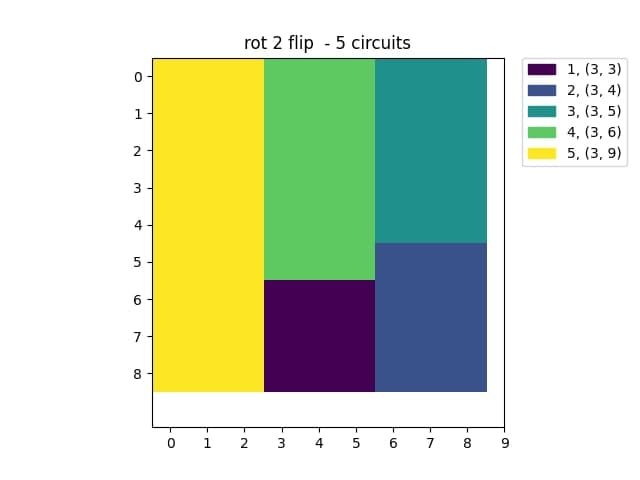
\includegraphics[width=2.5in]{images/sym_example/180_flipped.jpg} \\
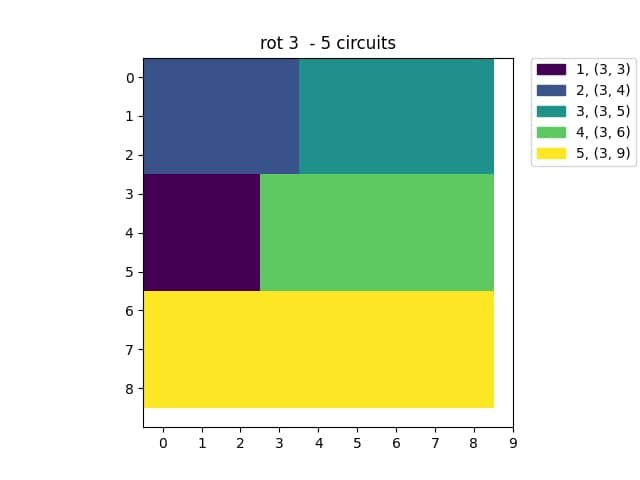
\includegraphics[width=2.5in]{images/sym_example/270.jpg} &
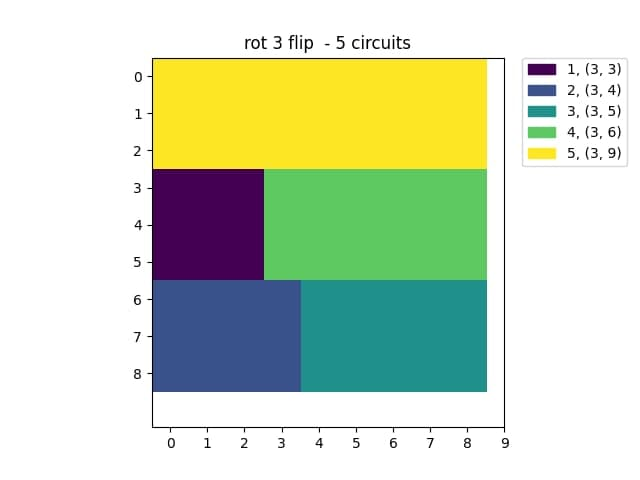
\includegraphics[width=2.5in]{images/sym_example/270_flipped.jpg} \\
\end{array}$
\end{center}
\caption{Second instance - all possible symmetric variants of a solution. Rot X indicates that the plate has undergone a rotation of X*90 degrees.}
\label{fig:symmetries}
\end{figure}

We could reduce the solver's work by reducing the number of solutions, thus by keeping only the non-symmetric ones. This can be done by placing the circuit with the largest area in the left-hand quarter of the silicon plate, namely by saying that $x_{big} \leq \dfrac{WIDTH}{2}$ and $y_{big} \leq \dfrac{HEIGHT}{2}$. This could be easily done in MiniZinc by adding this particular constraint:
\begin{lstlisting}[language=Mzn]
constraint symmetry_breaking_constraint(
    % This breaks the symmetries on the vertical axis
    corner_coords[biggest(), 1] * 2 <= width
    % This breaks the symmetries on the horizontal axis
    /\ corner_coords[biggest(), 2] * 2 <= height
    );
\end{lstlisting}
By looking at the figure \ref{fig:symmetries}, after the evaluation of the \textit{symmetry breaking constraint} the only solutions kept are 2 over the original 4, in the case we are not allowing rotation, whilst 4 over 8, in case of rotation.\\
A stronger \textit{symmetry breaking constraint} will place the biggest circuit in the lower-left corner of the silicon plate, namely in $(0,0)$:
$$x_{big} == 0 \land y_{big} == 0.$$
Nevertheless this constraint would not likely produce the desired effects, often slowing the solving process done by the MiniZinc's solver and as such it will not be considered in the CSP models comparison. The relative implementation is pretty straightforward:
\begin{lstlisting}[language=Mzn]
constraint symmetry_breaking_constraint(
    corner_coords[biggest(), 1] = 0
    /\ corner_coords[biggest(), 2] = 0
    );
\end{lstlisting}
\subsection{MiniZinc models comparisons}
The different models presented so far are now compared using a predefined configuration of the solver in order to avoid randomness in the results.
\\
\begin{table}[!h]
    \begin{tabular}{|c| p{2cm} | p{2 cm} | p{1.5cm} | c | c |}\hline
        Model &Rotation& Symmetry breaking& Solved instance & Mean time / instance (s) & Total time* (s) \\\hline
           1.0.0 & No  & No  & 23  & 30.79  & 708.20 \\ \hline
           1.3.0 & No  & No  & 25  & 6.86  & 171.56 \\ \hline
           1.0.0 & Yes & No  & 14  & 25.15 & 352.07 \\ \hline
           1.3.0 & Yes & No  & 17  & 43.59 & 741.02 \\ \hline
           1.0.0 & No  & Yes & 14  & 35.37  & 495.19 \\ \hline
           1.3.0 & No  & Yes & 22  & 21.19 & 466.13 \\ \hline
           1.0.0 & Yes & Yes & 21  & 26.32 & 552.82 \\ \hline
           1.3.0 & Yes & Yes & 26  & 17.48  & 454.53\\ \hline
    \end{tabular}
    \caption{MiniZinc models performances. Model 1.0.0 is the model without any global constraint, model 1.3.0 is the one with \texttt{diffn} and \texttt{cumulative}. (\emph{*}) the total time is computed by summing up successfully solved times.}
    \label{tab:csp-performance}
\end{table}

The best model is the \emph{1.3.0} the one with rotation and symmetry breaking, we think this is caused by the optimization done by the solver when we are using global constraints implemented in Minizinc. 
For further details, you can consult the file pdf \textbf{CSP\_performance.pdf}
\clearpage